%\clearpage%
%\ifodd\value{page}\hbox{}\newpage\fi%
\cleardoublepage

\thispagestyle{empty}%
\centering{
\vspace*{15mm}

\includegraphics[width=.90\textwidth]{bowling0.pdf}
\vspace*{25mm}


\includegraphics[width=.90\textwidth]{bowling1.pdf}
\par
}

\clearpage

\begin{center}
{\Huge Plusieurs activités sont financées par la}
\vspace*{5mm}
\par

\includegraphics[width=0.85\textwidth]{regie_fribourg.pdf}
\end{center}

\vfill
\begin{center}
	{\Huge et}
\end{center}
\vfill

\begin{center}
{\Huge par les comités de la Saint Nicolas\vspace*{1mm}\\
du Collège St-Michel}
\vspace*{5mm}
\par

\includegraphics[width=0.8\textwidth]{csm.jpg}
\end{center}


\clearpage
\thispagestyle{empty}%
\centering{
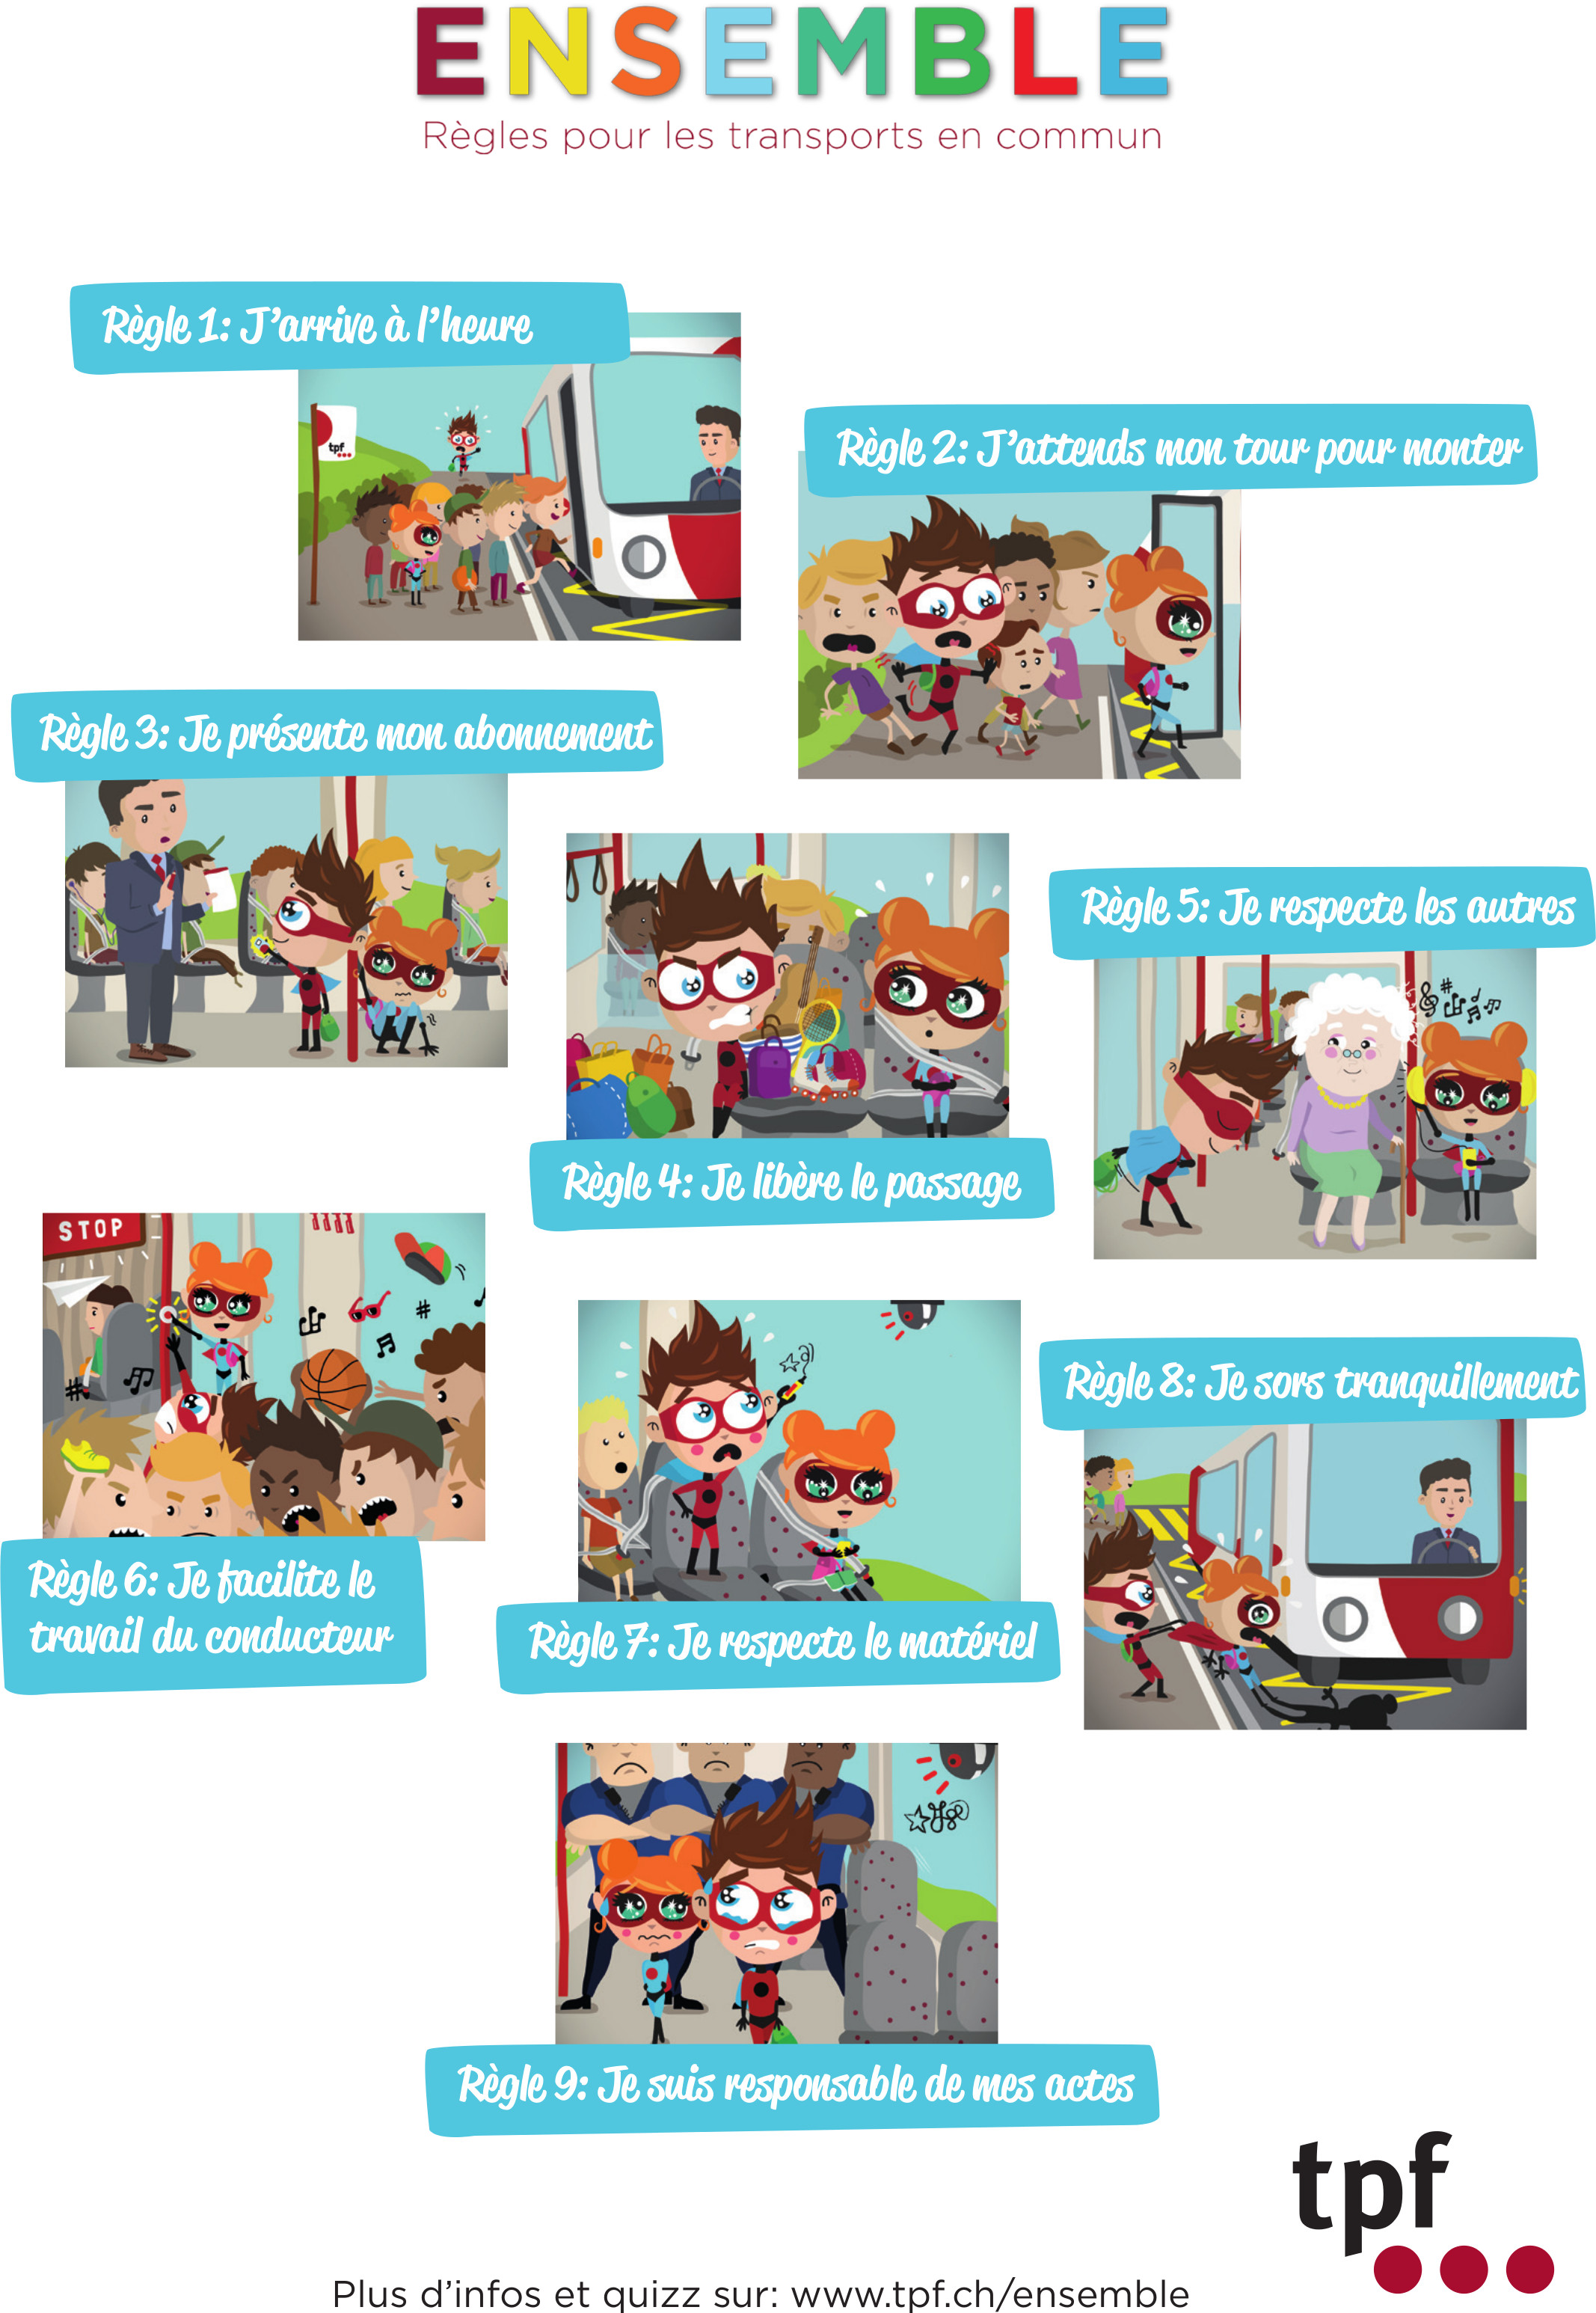
\includegraphics[width=.96\textwidth]{ensemble.jpg}
\par
}
\clearpage
\section*{Réseau régional\\Stadtnetz Regio}
\begin{textblock}{2}(11,1.3)

\includegraphics[width=3cm]{tpf.pdf}
\end{textblock}
\begin{center}
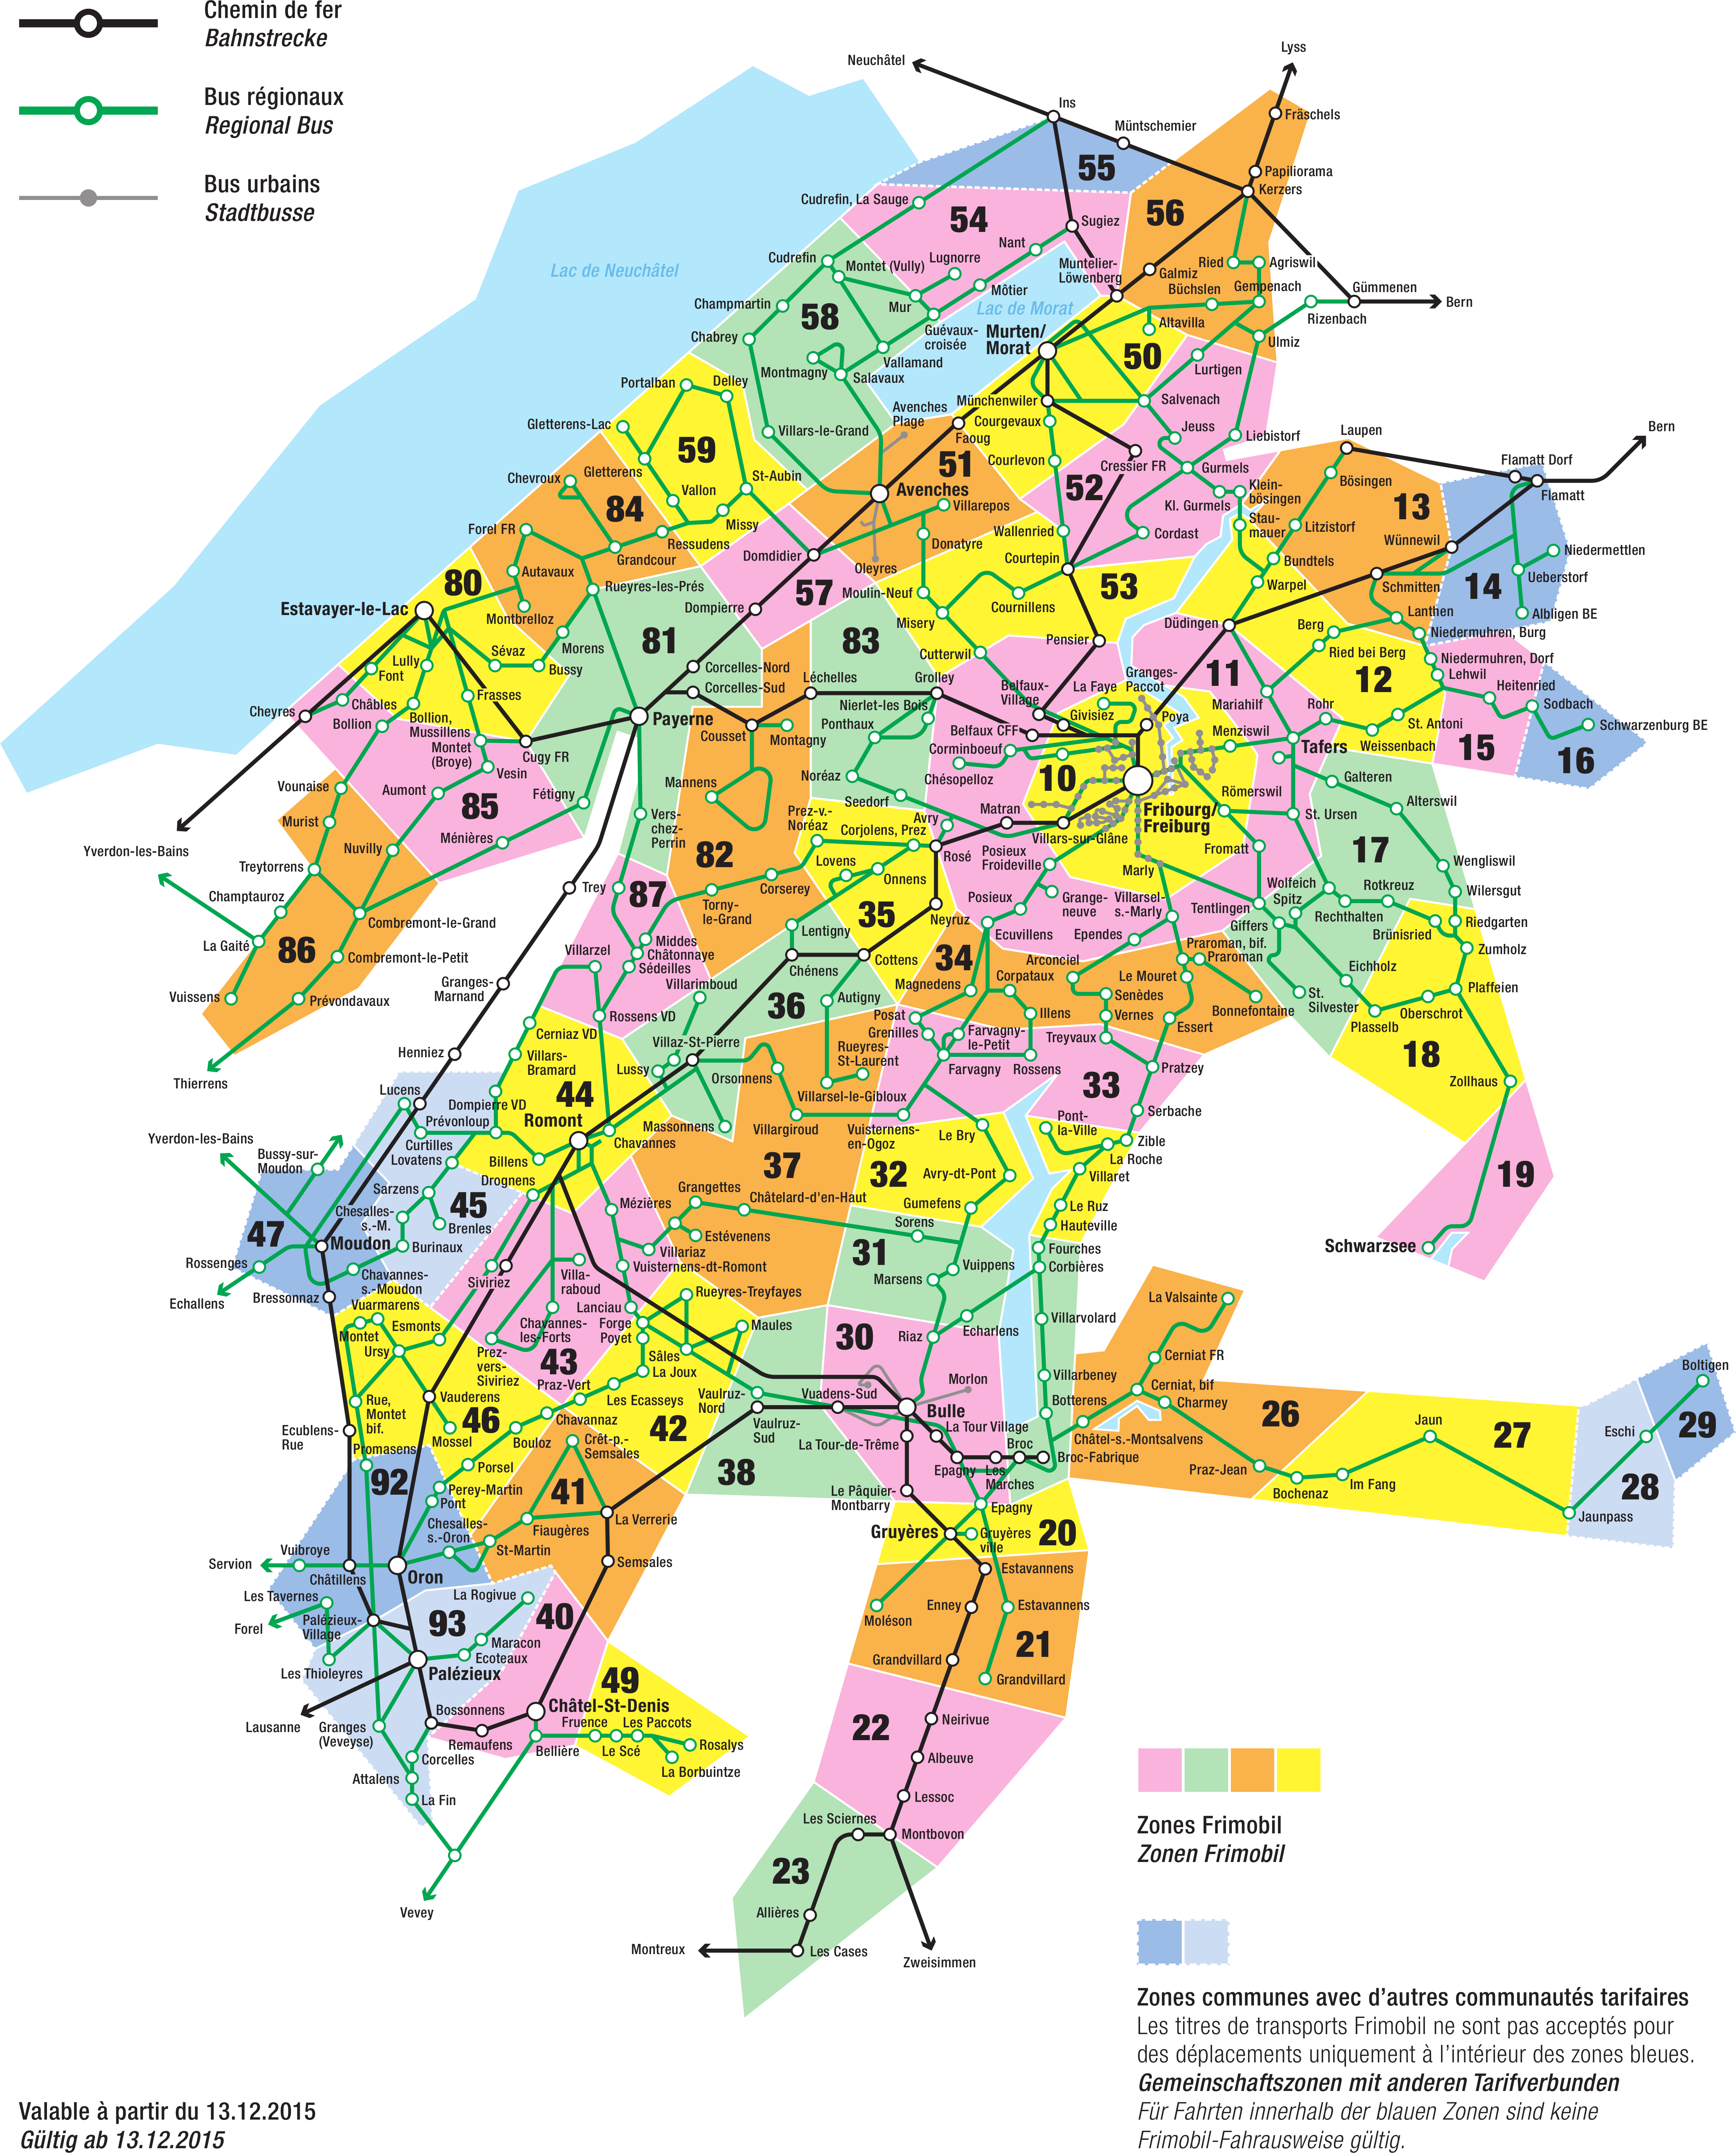
\includegraphics[width=\textwidth]{plan_regional.png}
\end{center}
\clearpage%
\thispagestyle{empty}%
\section*{Réseau Agglo Fribourg\\Stadtnetz Freiburg}%
\begin{textblock}{2}(11,1.3)%

\includegraphics[width=3cm]{tpf.pdf}%
\end{textblock}%
\begin{center}
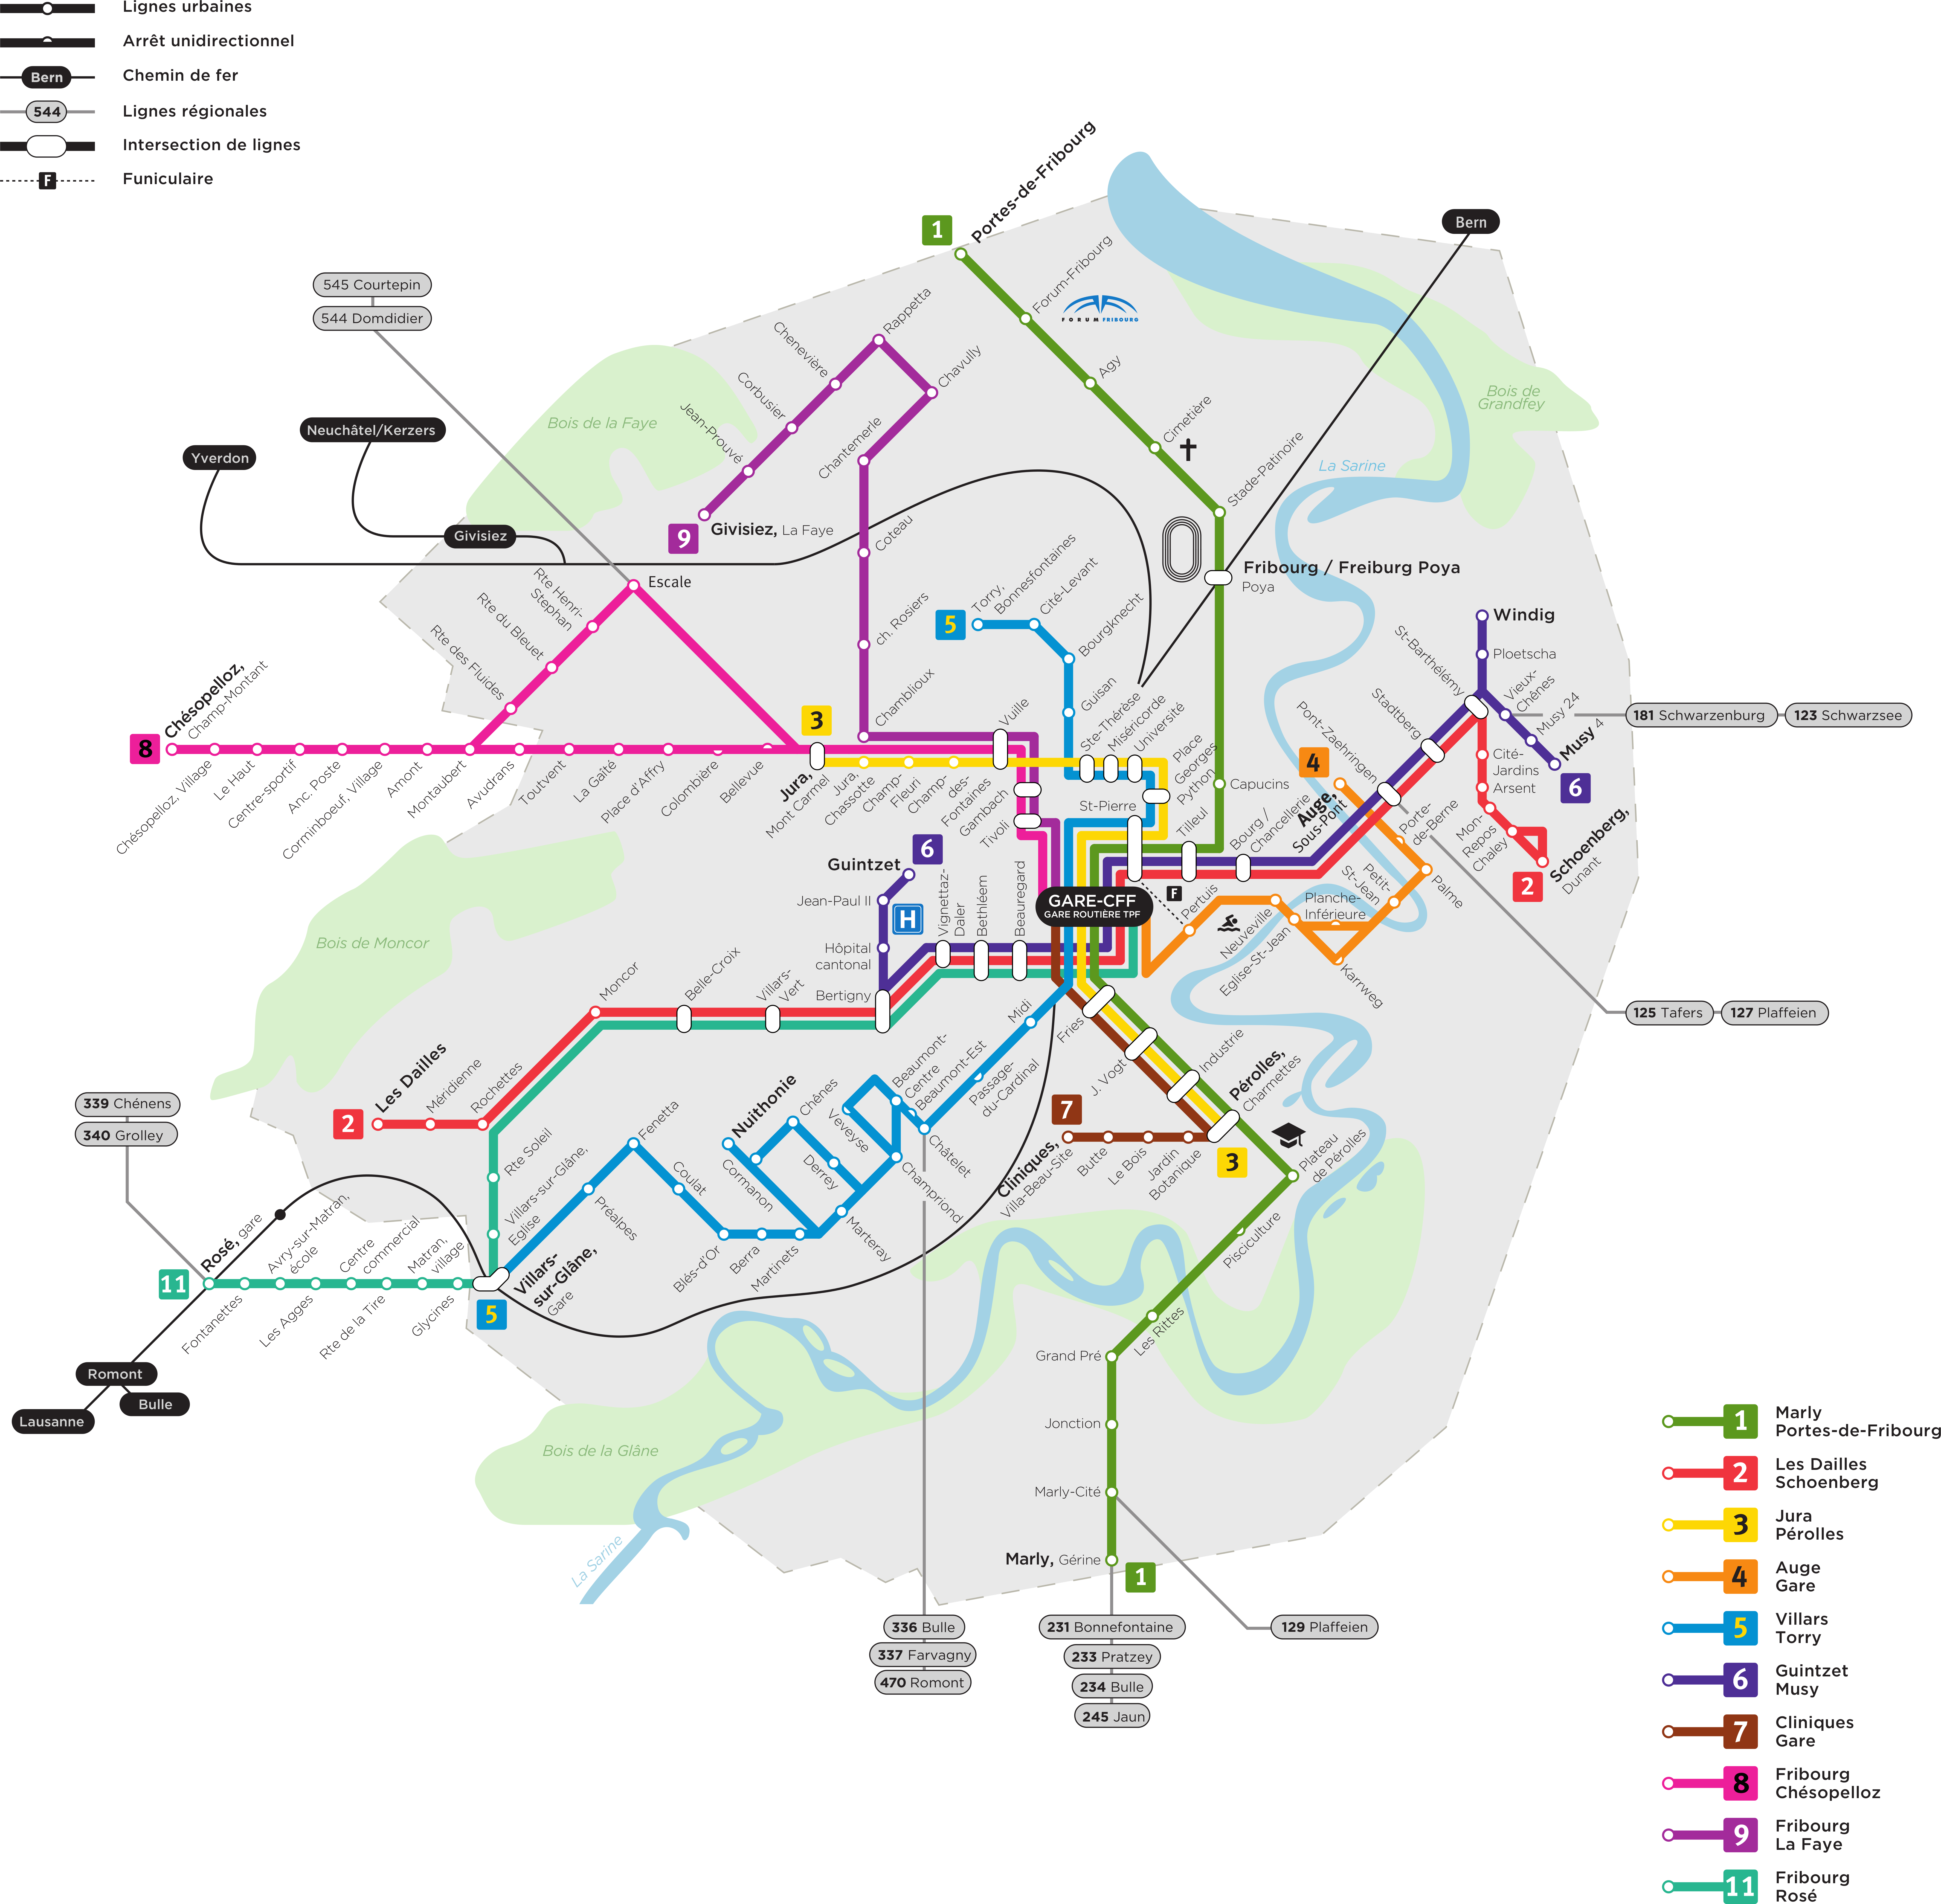
\includegraphics[width=\textwidth]{plan_zone_10.png}
\end{center}
